% Generated by make_fig_programs.py from programs/*.py and the study's code. Do not edit by hand.
\documentclass[border=3pt,varwidth=17.8cm]{standalone}
\usepackage{amsmath,amssymb,xcolor,listings,tikz}\usetikzlibrary{arrows.meta}
\definecolor{cblue}{HTML}{0072B2}\definecolor{cver}{HTML}{D55E00}\definecolor{cora}{HTML}{E69F00}\definecolor{cgreen}{HTML}{009E73}
\lstdefinestyle{qiskit}{language=Python,basicstyle=\ttfamily\tiny,numbers=left,numberstyle=\tiny\color{black!55},numbersep=3pt,keywordstyle=\color{cblue}\bfseries,commentstyle=\color{black!55}\itshape,showstringspaces=false,frame=single,rulecolor=\color{black!25},xleftmargin=9pt,framexleftmargin=9pt,columns=flexible,keepspaces=true}
\tikzset{gn/.style={circle,draw=black!70,fill=white,line width=0.4pt,minimum size=5.4mm,inner sep=0pt,font=\tiny},sl/.style={gn,fill=cblue!28}, spur/.style={gn,fill=cora!55}, cp/.style={draw=black,line width=1.3pt}, lin/.style={font=\fontsize{4.2}{5}\selectfont\color{black!60}},dataE/.style={-{Stealth[length=1.2mm]},draw=black!55,line width=0.45pt},quantumE/.style={-{Stealth[length=1.3mm]},draw=cblue,line width=0.9pt},controlE/.style={-{Stealth[length=1.3mm]},draw=cgreen,line width=0.8pt,dash pattern=on 2.2pt off 1.2pt},entE/.style={-{Stealth[length=1.2mm]},draw=cora,line width=0.6pt,dash pattern=on 1.2pt off 1pt}}
\begin{document}\begin{varwidth}{17.8cm}
\begin{minipage}[t]{0.27\linewidth}\vspace{0pt}{\footnotesize\textbf{(a) Teleportation}}\\[2pt]\lstinputlisting[style=qiskit,firstline=7,lastline=17,firstnumber=7]{programs/teleport.py}\end{minipage}\hfill
\begin{minipage}[t]{0.71\linewidth}\vspace{0pt}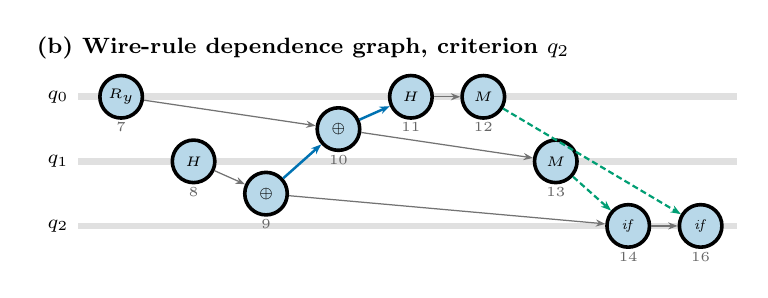
\begin{tikzpicture}
\begin{scope}[xshift=0.0cm]
\node[anchor=west, font=\footnotesize\bfseries] at (-0.55,2.26) {(b) Wire-rule dependence graph, criterion $q_2$};
\draw[black!12, line width=2.4pt] (0.1,1.64) -- (8.464,1.64); \node[anchor=east, font=\scriptsize] at (0.1,1.64) {$q_0$};
\draw[black!12, line width=2.4pt] (0.1,0.82) -- (8.464,0.82); \node[anchor=east, font=\scriptsize] at (0.1,0.82) {$q_1$};
\draw[black!12, line width=2.4pt] (0.1,0.0) -- (8.464,0.0); \node[anchor=east, font=\scriptsize] at (0.1,0.0) {$q_2$};
\node[sl,cp] (na0) at (0.644,1.640) {$R_y$};
\node[lin] at (0.644,1.250) {7};
\node[sl,cp] (na1) at (1.564,0.820) {$H$};
\node[lin] at (1.564,0.430) {8};
\node[sl,cp] (na2) at (2.484,0.410) {$\oplus$};
\node[lin] at (2.484,0.020) {9};
\node[sl,cp] (na3) at (3.404,1.230) {$\oplus$};
\node[lin] at (3.404,0.840) {10};
\node[sl,cp] (na4) at (4.324,1.640) {$H$};
\node[lin] at (4.324,1.250) {11};
\node[sl,cp] (na5) at (5.244,1.640) {$M$};
\node[lin] at (5.244,1.250) {12};
\node[sl,cp] (na6) at (6.164,0.820) {$M$};
\node[lin] at (6.164,0.430) {13};
\node[sl,cp] (na7) at (7.084,0.000) {$\mathit{if}$};
\node[lin] at (7.084,-0.390) {14};
\node[sl,cp] (na8) at (8.004,0.000) {$\mathit{if}$};
\node[lin] at (8.004,-0.390) {16};
\draw[dataE] (na0) to (na3);
\draw[dataE] (na1) to (na2);
\draw[quantumE] (na2) to (na3);
\draw[dataE] (na2) to (na7);
\draw[quantumE] (na3) to (na4);
\draw[dataE] (na3) to (na6);
\draw[dataE] (na4) to (na5);
\draw[controlE] (na5) to (na8);
\draw[controlE] (na6) to (na7);
\draw[dataE] (na7) to (na8);
\end{scope}
\end{tikzpicture}\\[1pt]\scriptsize def-use: 4 ops, lines 8, 9, 14, 16, $F=0.50$\quad classical PDG = wire: 9 ops, lines 7, 8, 9, 10, 11, 12, 13, 14, 16, $F=1.00$
\end{minipage}\\[8pt]
\begin{minipage}[t]{0.27\linewidth}\vspace{0pt}{\footnotesize\textbf{(c) VQE ansatz}}\\[2pt]\lstinputlisting[style=qiskit,firstline=5,lastline=17,firstnumber=5]{programs/ansatz.py}\end{minipage}\hfill
\begin{minipage}[t]{0.71\linewidth}\vspace{0pt}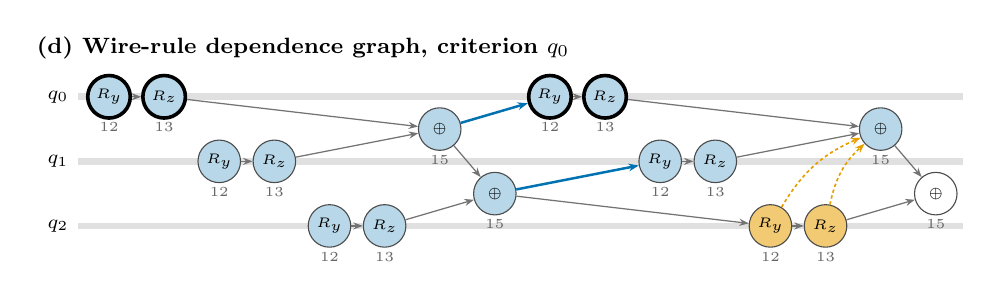
\begin{tikzpicture}
\begin{scope}[xshift=0.0cm]
\node[anchor=west, font=\footnotesize\bfseries] at (-0.55,2.26) {(d) Wire-rule dependence graph, criterion $q_0$};
\draw[black!12, line width=2.4pt] (0.1,1.64) -- (11.339999999999998,1.64); \node[anchor=east, font=\scriptsize] at (0.1,1.64) {$q_0$};
\draw[black!12, line width=2.4pt] (0.1,0.82) -- (11.339999999999998,0.82); \node[anchor=east, font=\scriptsize] at (0.1,0.82) {$q_1$};
\draw[black!12, line width=2.4pt] (0.1,0.0) -- (11.339999999999998,0.0); \node[anchor=east, font=\scriptsize] at (0.1,0.0) {$q_2$};
\node[sl,cp] (nb0) at (0.490,1.640) {$R_y$};
\node[lin] at (0.490,1.250) {12};
\node[sl,cp] (nb1) at (1.190,1.640) {$R_z$};
\node[lin] at (1.190,1.250) {13};
\node[sl] (nb2) at (1.890,0.820) {$R_y$};
\node[lin] at (1.890,0.430) {12};
\node[sl] (nb3) at (2.590,0.820) {$R_z$};
\node[lin] at (2.590,0.430) {13};
\node[sl] (nb4) at (3.290,0.000) {$R_y$};
\node[lin] at (3.290,-0.390) {12};
\node[sl] (nb5) at (3.990,0.000) {$R_z$};
\node[lin] at (3.990,-0.390) {13};
\node[sl] (nb6) at (4.690,1.230) {$\oplus$};
\node[lin] at (4.690,0.840) {15};
\node[sl] (nb7) at (5.390,0.410) {$\oplus$};
\node[lin] at (5.390,0.020) {15};
\node[sl,cp] (nb8) at (6.090,1.640) {$R_y$};
\node[lin] at (6.090,1.250) {12};
\node[sl,cp] (nb9) at (6.790,1.640) {$R_z$};
\node[lin] at (6.790,1.250) {13};
\node[sl] (nb10) at (7.490,0.820) {$R_y$};
\node[lin] at (7.490,0.430) {12};
\node[sl] (nb11) at (8.190,0.820) {$R_z$};
\node[lin] at (8.190,0.430) {13};
\node[spur] (nb12) at (8.890,0.000) {$R_y$};
\node[lin] at (8.890,-0.390) {12};
\node[spur] (nb13) at (9.590,0.000) {$R_z$};
\node[lin] at (9.590,-0.390) {13};
\node[sl] (nb14) at (10.290,1.230) {$\oplus$};
\node[lin] at (10.290,0.840) {15};
\node[gn] (nb15) at (10.990,0.410) {$\oplus$};
\node[lin] at (10.990,0.020) {15};
\draw[dataE] (nb0) to (nb1);
\draw[dataE] (nb1) to (nb6);
\draw[dataE] (nb2) to (nb3);
\draw[dataE] (nb3) to (nb6);
\draw[dataE] (nb4) to (nb5);
\draw[dataE] (nb5) to (nb7);
\draw[dataE] (nb6) to (nb7);
\draw[quantumE] (nb6) to (nb8);
\draw[quantumE] (nb7) to (nb10);
\draw[dataE] (nb7) to (nb12);
\draw[dataE] (nb8) to (nb9);
\draw[dataE] (nb9) to (nb14);
\draw[dataE] (nb10) to (nb11);
\draw[dataE] (nb11) to (nb14);
\draw[dataE] (nb12) to (nb13);
\draw[dataE] (nb13) to (nb15);
\draw[dataE] (nb14) to (nb15);
\draw[entE] (nb12) to[bend left=18] (nb14);
\draw[entE] (nb13) to[bend left=18] (nb14);
\end{scope}
\end{tikzpicture}\\[1pt]\scriptsize classical PDG: 4 ops, lines 12, 13, $F=0.77$\quad QPDG: +2 non-dependences\quad wire: 13 ops $=$ dependences, $F=1.00$
\end{minipage}\\[6pt]
\centering\scriptsize\tikz\draw[dataE](0,0)--(0.5,0); data\quad \tikz\draw[controlE](0,0)--(0.5,0); control\quad\tikz\draw[quantumE](0,0)--(0.5,0); quantum, missing from the classical PDG\quad\tikz\draw[entE](0,0)--(0.5,0); entanglement closure (QPDG)\\\tikz\node[sl,minimum size=3mm]{}; wire slice\quad \tikz\node[gn,cp,minimum size=3mm]{}; classical PDG slice\quad\tikz\node[spur,minimum size=3mm]{}; added by QPDG, not a dependence\quad small numbers: source line
\end{varwidth}\end{document}
